%TODO: Talk about how transactions can be composed.
% We 'll need to do this for the PIFO work as well.

\section{Packet transactions}
\label{s:transactions}

\begin{figure*}[!t]
\begin{minipage}{0.5\textwidth}
\begin{small}
\begin{lstlisting}[style=customc]
#define NUM_FLOWLETS    8000
#define THRESHOLD       5
#define NUM_HOPS        10

struct Packet {
  int sport;
  int dport;
  int new_hop;
  int arrival;
  int next_hop;
  int id; // array index
};

int last_time [NUM_FLOWLETS] = {0};
int saved_hop [NUM_FLOWLETS] = {0};

void flowlet(struct Packet pkt) {
  pkt.new_hop = hash3(pkt.sport,
                      pkt.dport,
                      pkt.arrival)
                % NUM_HOPS;

  pkt.id  = hash2(pkt.sport,
                  pkt.dport)
            % NUM_FLOWLETS;

  if (pkt.arrival - last_time[pkt.id] @\label{line:ifStart}@
      > THRESHOLD)
  { saved_hop[pkt.id] = pkt.new_hop; } @\label{line:ifEnd}@

  last_time[pkt.id] = pkt.arrival;
  pkt.next_hop = saved_hop[pkt.id];
}
\end{lstlisting}
\end{small}
\caption{Flowlet switching written in \pktlanguage}
\label{fig:flowlet_code}
\end{minipage}
%
\vrule\quad
%
\begin{minipage}{0.4\textwidth}
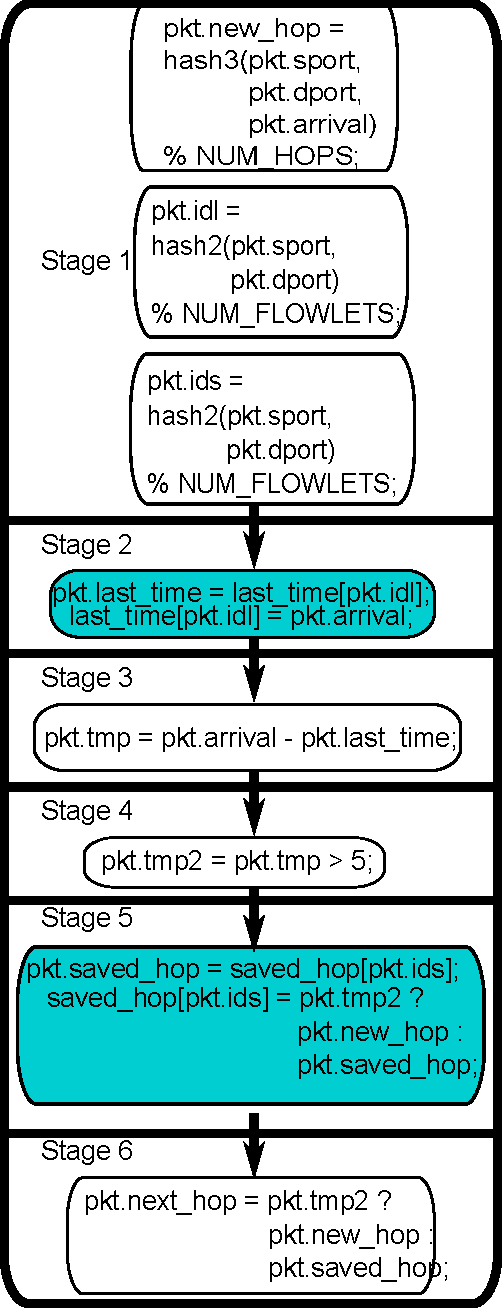
\includegraphics[width=0.8\columnwidth]{pipe.pdf}
\caption{Compiled 6-stage \absmachine pipeline implementing flowlet
switching.  Control flows from top to bottom. Atoms manipulating state are
shaded in blue.}
\label{fig:flowlet_pipeline}
\end{minipage}
\end{figure*}

We now illustrate programming using packet transactions in \pktlanguage, using
flowlet switching~\cite{flowlets} as an example. Flowlet switching is a
load-balancing algorithm that sends bursts of packets (called flowlets) from a
TCP flow on different paths, provided the bursts are separated by a large
enough interval in time to ensure packets do not arrive out of order at a TCP
receiver. Figure~\ref{fig:flowlet_code} shows flowlet switching as expressed in
\pktlanguage. For simplicity, the example hashes only the source and
destination ports; it is easy to extend it to the full 5-tuple.

This example demonstrates the core language constructs in \pktlanguage. All
packet processing happens in the context of a packet transaction (the function
\texttt{flowlet} starting at line 17). The function's argument {\tt pkt}
declares the fields in a packet (lines 5--12)\footnote{We use fields to refer
to both packet headers such as source port ({\tt sport}) and destination port
({\tt dport}) and packet metadata ({\tt id}).} that can be referenced by the
function body (lines 18--32).  The function body can also reference persistent
state stored on the switch using global variables (e.g.  \texttt{last\_time}
and \texttt{saved\_hop} on lines 14 and 15, respectively).

Conceptually, the switch invokes the packet transaction function on each
incoming packet sequentially. To the programmer, the function modifies the
passed-in packet argument and runs to completion before processing the next
packet.  The function may invoke \textit{intrinsics} such as \texttt{hash2} on
line 23 to use hardware accelerators such as hash generators.  The \pktlanguage
compiler uses an intrinsic's signature to infer dependencies and supplies a
canned run-time implementation, but otherwise does not analyze an intrinsics's
internal behavior.

\subsection{Constraints on the language}
%%\pktlanguage relative to software
%%routers like Click~\cite{click} with greater flexibility and variable
%%performance.

The overall language is a constrained subset of C (Table~\ref{tab:restrict}).
These constraints are required for deterministic performance.  Memory
allocation, unbounded iteration counts, and unstructured control flow all cause
variable performance, which may prevent an algorithm from running at line rate.
Arrays can be used as state variables alone but not as packet fields.
Furthermore, all accesses to a given array within one execution of a
transaction, i.e. one packet, must use the same array index. For instance, all
read and write accesses to the array \texttt{last\_time} use the index
\texttt{pkt.id}, which is constant for each packet, but can change from one
packet to the next. This restriction mirrors restrictions on memories, where
supporting distinct read and write addresses every clock cycle is challenging.

\begin{table}
  \begin{tabular}{p{0.9\columnwidth}}
    No iteration (while, for, do-while).\\
    No goto, break, or continue.\\
    No pointers.\\
    No dynamic memory allocation / heap.\\
    Array index is constant for each transaction execution.\\
    No access to data i.e. unparsed portion of the packet.\\
    No arrays in packet fields.\\
  \end{tabular}
  \caption{Restrictions in \pktlanguage}
  \label{tab:restrict}
\end{table}

\subsection{All-or-nothing compilation}

When compiled to a \absmachine machine (\S\ref{s:absmachine}), the \pktlanguage
compiler (\S\ref{s:compiler}) converts the code in
Figure~\ref{fig:flowlet_code} into the atom pipeline shown in
Figure~\ref{fig:flowlet_pipeline}. The compiler guarantees that code accepted
by the compiler can run at line rate on the abstract machine or rejects it
outright; there is no smooth tradeoff between a program's performance and its
complexity.

The all-or-nothing compilation model is unusual for someone programming other
computational substrates such as a CPU, GPU, or DSP. But, it reflects how
routers and switches have always been used. Routers are rated for a particular
line rate, regardless of the feature set that is enabled. The all-or-nothing
model provides predictable performance for free---in contrast to
software-router platforms that need to be explicitly architected for
predictability~\cite{dobrescu2012, wenfei15}.

\subsection{Limitations of packet transactions}

Packet transactions are a good fit for data-plane algorithms that do a small
amount of work per packet (i.e. where the amount of work can be bounded at
compile time) and manipulate only packet headers. Data-plane algorithms like
deep packet inspection and wan optimization access packet payloads. These
algorithms require a switch to parse not just packet headers, but the packet
payload as well---effectively parsing a huge header consisting of each byte in
the packet payload. Parsing such deep parse graphs is challenging at line rates
of 1 GHz. Consequently, the limitations of packet transactions merely reflect
fundamental limitations of the underlying hardware.
